\begin{figbox}{!t}
\caption{Culture, belonging, values and fairness at CSIT}
\label{fig:treated2}

\sffamily
\footnotesize
\RaggedRight

\begin{tabular}{p{3.3cm} !{\quad} p{11cm}}
\addlinespace 

The prevailing culture and atmosphere in the school is inclusive and friendly to all & 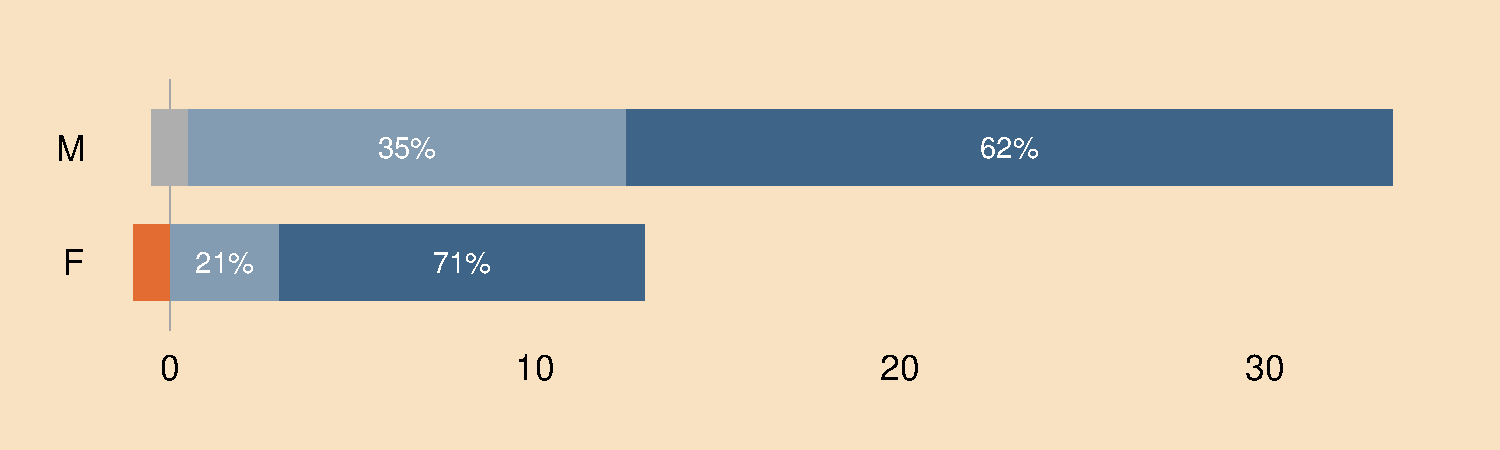
\includegraphics[align=t,trim={0 0 0 15mm},clip,width=11cm]{fig/culture/paolo5.pdf}\\

\hdashline

Do you feel that you belong to the school? & 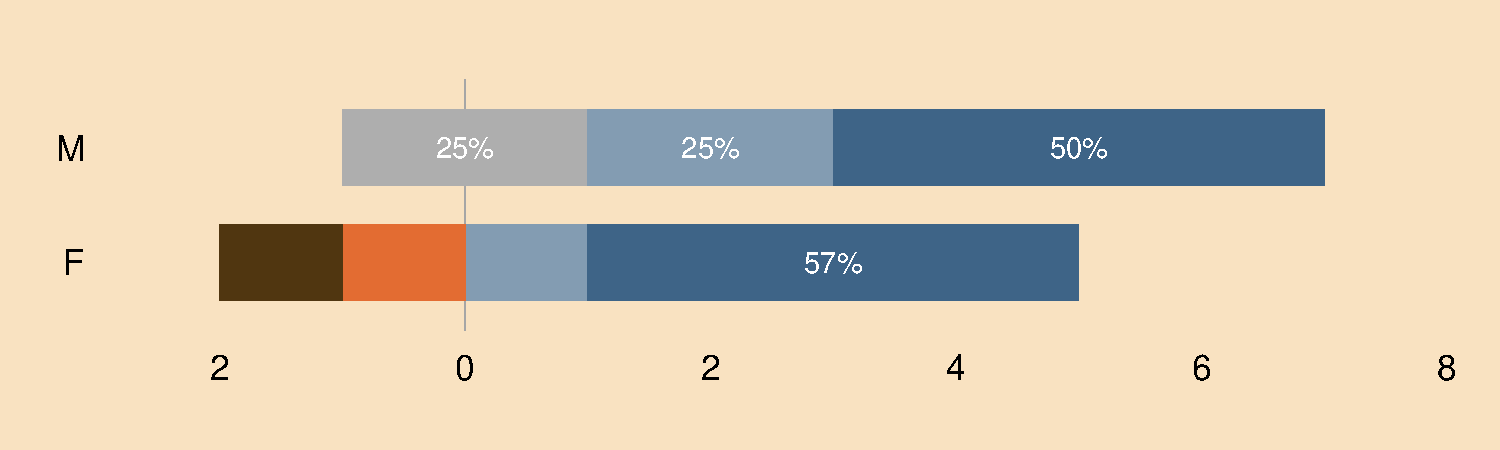
\includegraphics[align=t,trim={0 0 0 15mm},clip,width=11cm]{fig/culture/paolo6.pdf}\\

\hdashline

The school promotes clear values and expectations about how people should behave towards each other & 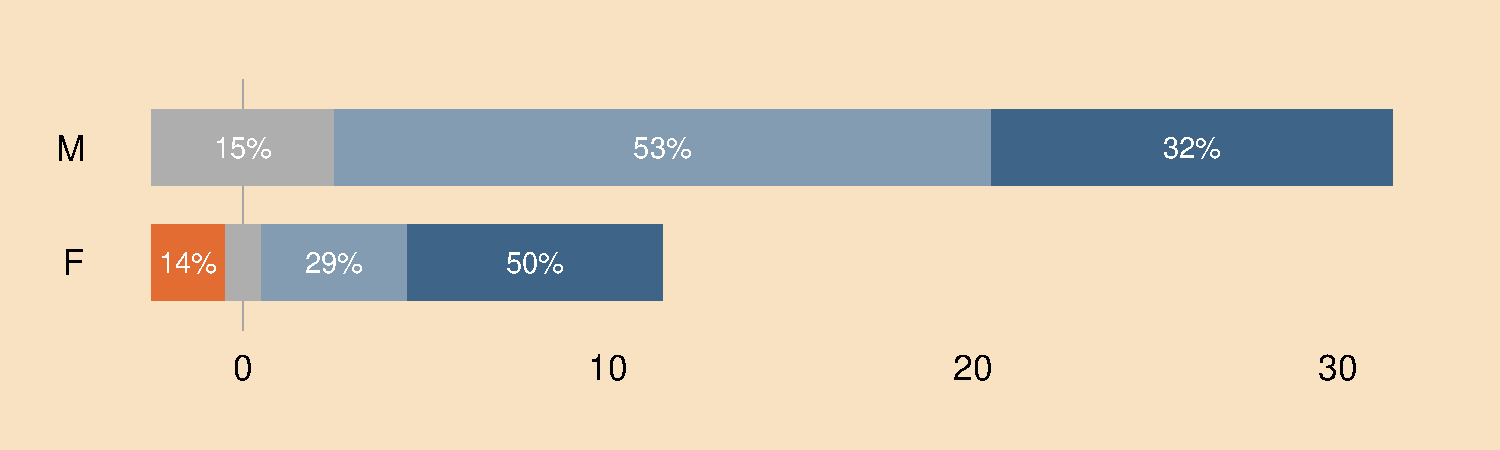
\includegraphics[align=t,trim={0 0 0 15mm},clip,width=11cm]{fig/culture/paolo7.pdf}\\

\hdashline

I am treated fairly, based on merit, without regard to characteristics of gender, civil or family status, sexual orientation, religion, age, disability, race or membership of the Traveller community & 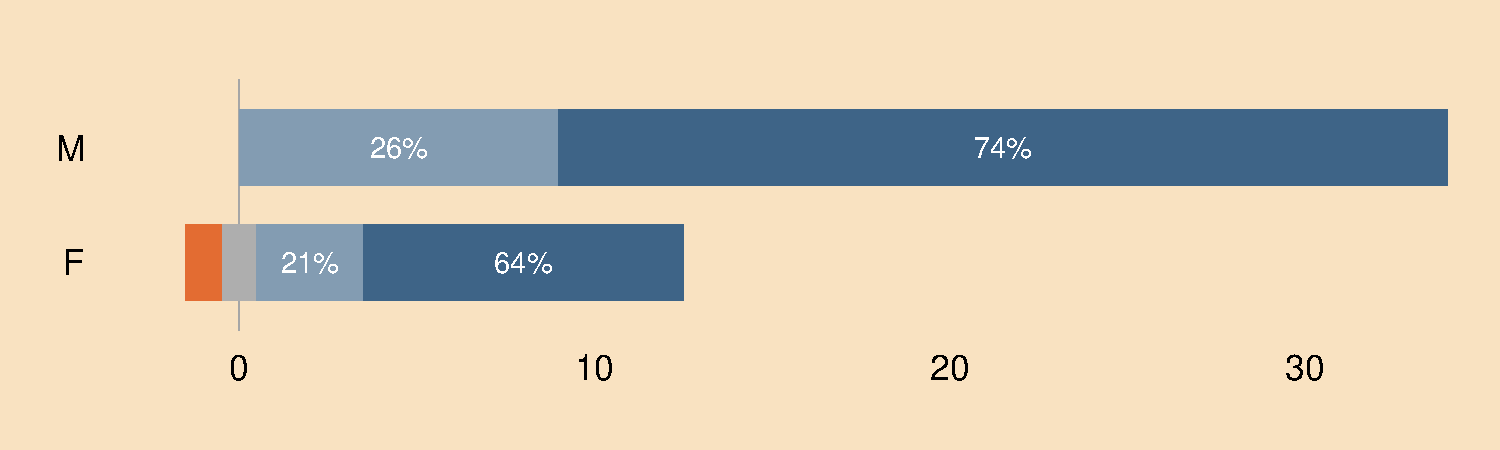
\includegraphics[align=t,trim={0 0 0 15mm},clip,width=11cm]{fig/culture/paolo8.pdf}\\

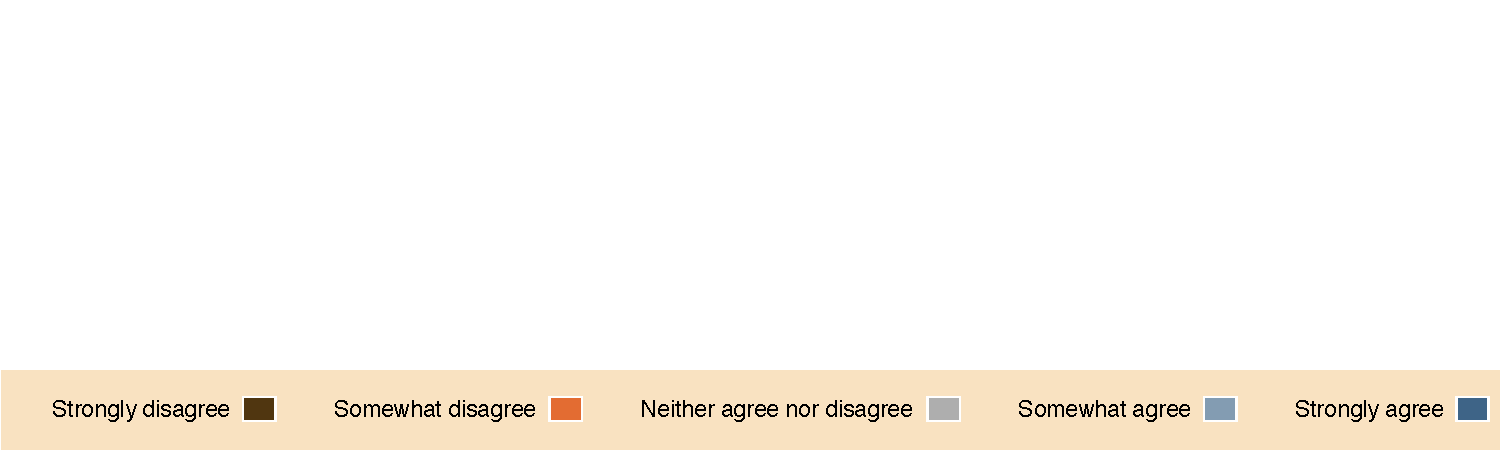
\includegraphics[trim={6mm 0 0 0},clip,width=14.5cm]{fig/legend5col.pdf}\\

\end{tabular}
\end{figbox}